\documentclass{report}
\usepackage{graphicx}
\usepackage{wasysym}
\usepackage{listings}
\usepackage{color}
\usepackage{multirow}

\graphicspath{{test_results/}}

\newcommand*\cbox{\item[\XBox]}
\newcommand*\uncbox{\item[\Square]}

\definecolor{dkgreen}{rgb}{0,0.6,0}
\definecolor{gray}{rgb}{0.5,0.5,0.5}
\definecolor{mauve}{rgb}{0.58,0,0.82}

\lstset{frame=tb,
  language=Python,
  aboveskip=3mm,
  belowskip=3mm,
  showstringspaces=false,
  columns=flexible,
  basicstyle={\small\ttfamily},
  numbers=none,
  numberstyle=\tiny\color{gray},
  keywordstyle=\color{blue},
  commentstyle=\color{dkgreen},
  stringstyle=\color{mauve},
  breaklines=true,
  breakatwhitespace=true,
  tabsize=3
}


\begin{document}


\section{Energy-based models}

\subsection{Restricted Boltzmann Machines}	
cite{video slides}
Not a causal generative model, but is instead defined in terms of the energies of joint configurations of the visible and hidden units. These energies can be translated into their probabilities in two ways: 
\begin{itemize}
	\item $p(v, h) \propto e^{-E(v, h)}$
	\item Multiple update of units, then define the probability of the probability of finding the network in that joint configuration.
\end{itemize}

\paragraph{Using energies to define probabilities}
\begin{equation}
p(v, h) = \frac{e^{-E(v, h)}}{\displaystyle\sum_{u, g}e^{-E(u, g)}}
\end{equation}

where the probability of a joint configuration depends on the energy compared with the energy of all other joint configurations. The denominator is also known as the partition function (a normalizing constant to ensure the probability distribution sums up to 1).

Inference and learning is easier than regular Boltzmann Machines by restricting the connectivity (no connections between hidden units). Since the units are independent, the probabilities can be calculated all in parallel. In the positive phase, $v_i h_j$ is computed for all pairs (the exact value of $h_j$ can be easily computed as a datavector when clamped on the visible units). Then $v_i h_j$ is averaged over all data in the mini-batch. After backwards feeding, forward feeding is performed with the probability input, rather than the reconstructed input. The drawbacks is that you only have one hidden layer.

In the negative phase, you have a set of "fantasy particles" (a global configuration), which are updated a few times using alternating parallel updates. Then $v_i h_j$ is averaged over all fantasy particles.

\subsection{Stacked RBMs}
Stacking RBMs turns the output of the hidden layers to input for the next hidden layers. There can be as many hidden layers as desired, and together they compose a single, multilayer generative model and "each additional hidden layer improves a lower bound on the probability that the multilayer model would generate the training data." (check Hinton et al 2006). Features can be learnt from features in higher level representations.  


\subsection{DBN}
DBN classifier

\subsection{The Classifier and The MNIST dataset}
MNIST: classification and generation
The classifier has been trained on the MNIST dataset, a collection of handwritten digits as strongly bimodal input values. In the original dataset each pixel of the image is represented by a value between 0 and 255, where 0 is black, 255 is white and values in between are different shades of gray.

\section{Experiment}
\subsection{Classification}
To test the classifier for performance when dealing with possibly erroneous data, we added noise to the input data. The input data are vectors of 784 float values between 0 and 1, each corresponding to a pixel of a 28x28 digital representation of a handwritten digit, where 0 is black, and 1 is white. Noise is simulated by imputing the input vector with 1's at randomly chosen locations, based on a set percentage. 

% insert image of test digit and imputed test digit
\begin{figure}[h!]
	\begin{tabular}{c c}
	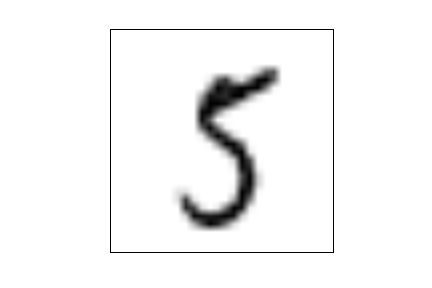
\includegraphics[width=.45\textwidth]{test_digit} & 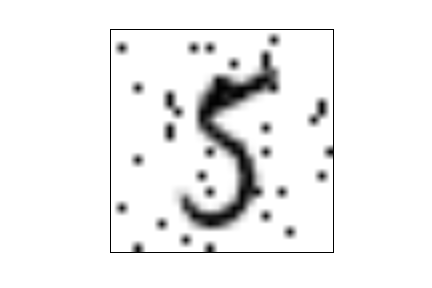
\includegraphics[width=.45\textwidth]{imp_test_digit}
	\end{tabular}
	\caption{An example of an inverted digitalized handwritten 5, and the same image randomly noised at 4\%.}
\end{figure}



The test data set contains 2000 image vectors. For a means of comparison, we tested the classifier on the original dataset and recorded the classification error rate, as well as the free energy ($\mathcal{F}$) using the formula above. The error rate is calculated by comparing the predicted class with the test set's corresponding y set. $\mathcal{F}$ is calculated for the whole network, so the total of each pair of visible and hidden layer's $\mathcal{F}$, plus that of the class layer. For the simulated noised dataset, each individual image vector is subject to random imputation, each time increasing the imputation by 1\%. The dataset is then reran through the classifier.  The table below shows the $\mathcal{F}$ mean for each set, and the classification error rate as the imputation percentage is incremented.

% insert table with imputed data, no reclassification. Maybe also confusion matrix
\begin{table}[h!]
	\begin{center}
		\begin{tabular}{c | c | c}
		\% imputation & $\mathcal{F}$ mean & error rate \\
		\hline
		0 & -397.24 & 0.13 \\
		1 & -348.88 & 0.15 \\
		2 & -294.55 & 0.20 \\
		3 & -244.50 & 0.26 \\
		4 & -197.98 & 0.37 \\
		5 & -155.40 & 0.48 \\
		6 & -116.56 & 0.57 \\
		7 & -82.21 & 0.65 \\
		8 & -45.98 & 0.69 \\
		9 & -13.79 & 0.76 \\
		10 & 19.82 & 0.80 \\
		
		\end{tabular}
	\end{center}
	\caption{$\mathcal{F}$ mean and classification error rate as noise is increased.}
\end{table}


\begin{figure}
\begin{center}
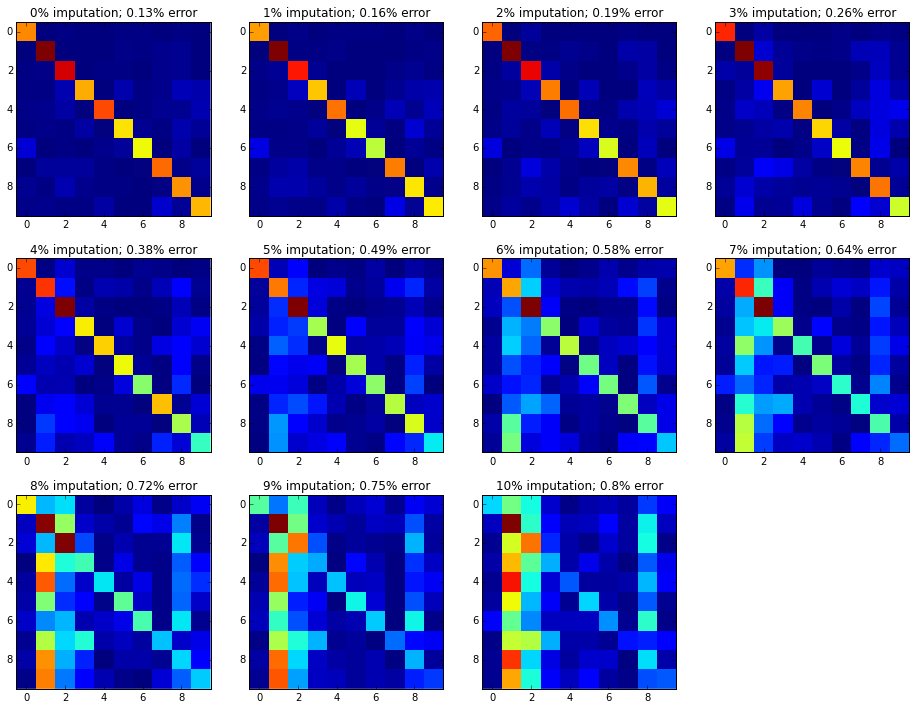
\includegraphics[width=\textwidth]{confusion_matrices}
\end{center}
\end{figure}


There are many techniques to discover if data is reliable, such as clustering for outlier detection, or [insert here], but we chose to inspect a measure that is specific to neural networks. As DBNs are a neural network of stacked RBMs, which are energy-based models, we analyzed the behaviour of $\mathcal{F}$ outside of its role in the training of the model. In training, the energy determines the probability of a joint configuration of the visible (here the pixels of the image vector) and hidden units, and is used in the definition of the model's learning. In testing, energy can be used as a marker for unexpected input data since it directly affected by the values of the visible layer. As expected, $\mathcal{F}$ evolves proportionally to the amount of added noise. 

\begin{figure}
	\centering
		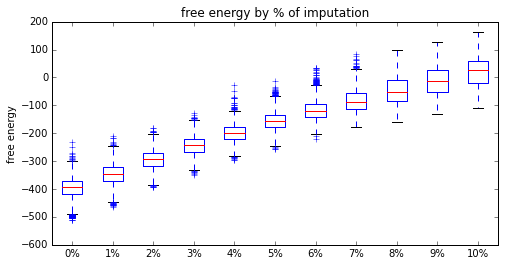
\includegraphics[width=\textwidth]{nrgs_bp}
	\caption{Free energies of each input vector as noise is increased}
\end{figure}


From the energy formula, we can see how the energy is directly affected. A deviation from the expected values of the input vector will be captured when going through the network and subject to its learned weights. This will raise the energy and act as a flag for an undesirable configuration, or in our case, noisy data.


\subsection{Reconstruction}
In an attempt to fix the noisy data, we look to the generative powers of the network to reconstruct the image vector. The issue here is that for the generation, the model must be provided a class to generate the desired digit. Our class is unknown, or rather unreliable, as seen from the increasing error rates, and the wrong class will generate the wrong digit. We therefore must choose a threshold to alert us when a predicted class cannot be trusted.


$\mathcal{F}$ is measured using arbitrary units, and its range is specific to each model. The threshold must therefore be chosen based on individual models. The maximum value of $\mathcal{F}$ yielded by the original, clean dataset, was chosen as the threshold for our classifier. If the calculated $\mathcal{F}$ of a given input vector is greater than the set threshold, it is sent back and reclassified n times. The prediction of each reclassification is stored and the class with the greatest count is then chosen as the class label to be clamped in the generation process. This new image is weighted, then fused with the original one, and rerun through the classifier. The results are shown in the table below.

\begin{table}
	\begin{center}
		\begin{tabular}{| c | r | c | c || c | c |}
		\cline{3-6}
		\multicolumn{2}{c|}{ } & \multicolumn{2}{c ||}{Reconstruction} & \multicolumn{2}{c|}{Reclassification}\\
		\hline
		 noise & n & $\mathcal{F}$ mean & error rate & $\mathcal{F}$ mean & error rate\\
		\hline
		    & 25 & -397.60 & 0.14 & -397.56& 0.13  \\
		0\% & 50 & -397.53 & 0.12 & -397.61 & 0.14 \\
		    & 100 & -397.63 & 0.12 & -397.19 & 0.14 \\
		    & 1000 & -243.06 & 0.13 & -397.19 & 0.14 \\
		 \hline
		    & 25 & -311.04 & 0.20 & -296.27 & 0.15 \\
		2\% & 50 & -311.89 & 0.19 & -296.25 & 0.14 \\
		    & 100 & -311.07 & 0.18 & -295.98 & 0.13 \\
		    & 1000 & -309.53 & 0.18 & -295.98 & 0.13 \\
		 \hline
		    & 25 & -314.16 & 0.43 & -155.55 & 0.12 \\
		5\% & 50 & -317.56 & 0.39 & -155.87 & 0.24 \\
		    & 100 & -315.58 & 0.38 & -156.14 & 0.25 \\
		    & 1000 & -317.4 & 0.39 & & \\
		 \hline
		     & 25 & -185.76 & 0.78 & 18.94 & 0.75 \\
		10\% & 50 & -185.92 & 0.79 & 20.26 & 0.74\\
		     & 100 & -191.98 & .80 & 19.97 & 0.74\\
		     & 1000 & \\
			
		\end{tabular}
	\end{center}
	\caption{\textbf{Reconstruction vs. Reclassification alone}: Mean of $\mathcal{F}$ and error rates by percentage of imputation and reclassification iterations}
\end{table}


We see an important drop in error rates not only in the classification with the mixed images, but also just with the reclassification alone.



\begin{figure}
	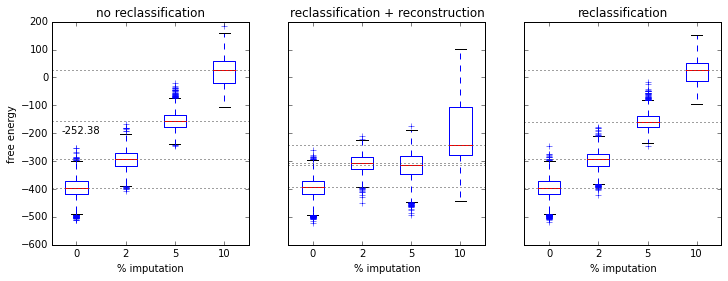
\includegraphics[width=\textwidth]{FE_boxplots}
	\caption{$\mathcal{F}$ measures for control set, reconstruction set, and reclassification alone set. -252.38 is the highest recorded $\mathcal{F}$ at 0\% imputation, and is set at threshold for unreliability.}
\end{figure}

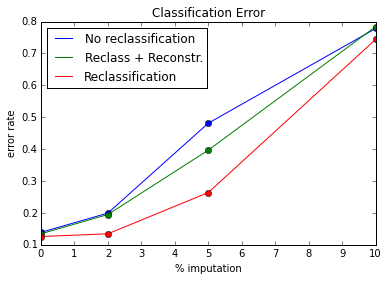
\includegraphics[width=0.7\textwidth]{err_plot}

The number of reclassification loops has an effect as well, and has been chosen based on the favourable results and the amount of time required. The optimal number of reclassification iterations was set to 50.

From the graphs, we can see that subjecting the noised images to reclassification yields better results in terms of error rate. However, if the goal is to reconstruct the input data to rid it of noise, the added reconstruction is also successful, as seen by both the error rates and the $\mathcal{F}$ measures.

, using the original noisy image and a generated, noiseless image

The mixing is to avoid the network classifying its own generations but also to emphasize the features that are to be detected by the network. This is done by applying a weight to the original image to pull out the important features amongst the noise, and the inverse of the weight vector to the generated image to pull out the noiseless features. The weight vector is built by taking the average of all training images. Below is an example of the mixing process.

% weight matrix, inv-weight matrix, imputed image, generated image, nw image, gw image, mixed. 
\begin{figure}
\begin{center}
\begin{tabular}{c  c}
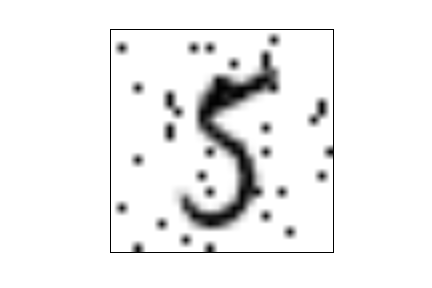
\includegraphics[width=0.4\textwidth]{imp_test_digit} & 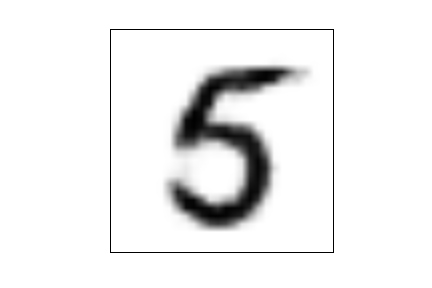
\includegraphics[width=0.4\textwidth]{generated} \\
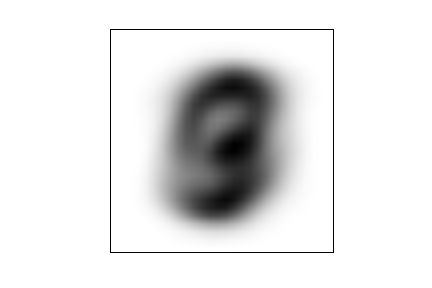
\includegraphics[width=0.4\textwidth]{weights} & 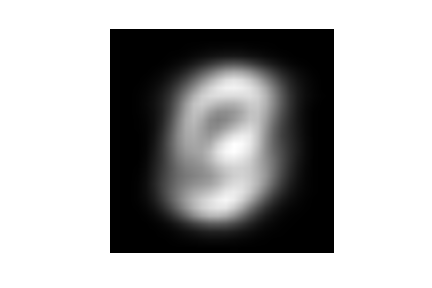
\includegraphics[width=0.4\textwidth]{inv_weights} \\
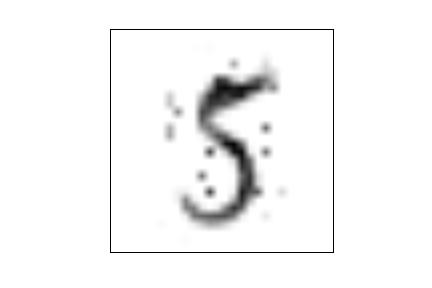
\includegraphics[width=0.4\textwidth]{nw} & 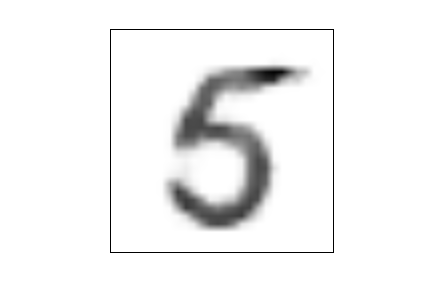
\includegraphics[width=0.4\textwidth]{gw} \\
\end{tabular}
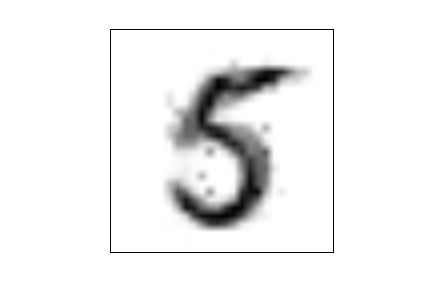
\includegraphics[width=0.4\textwidth]{mix}
\end{center}
\end{figure}


FE as marker for noise, noise as marker for unreliability
Generation to aid reconstruct unreliable data
Need correct class for generation, so do n-loops of classification, and choose class with highest count
Mix the weighted corrupted image with the weighted generated image


plot filters ?
\end{document}
